%************************************************************************
\section{Methodology}
\label{subsec:methodology}
% Explain the methods and techniques which will be used for your project depending on the subject: field work, laboratory work, modeling technique, interdisciplinary collaboration, data type, data acquisition, infrastructure, software, etc.
%************************************************************************
Specify the overall methodology you want to apply in order to reach your goals and answer your research questions. We often apply the HCD process (cf.~\autoref{fig:hcd}): 1. Vision, 2. Analyze, 3. Design for Usability, 4. Construct and Deploy (Implementation), 5. Evaluate in Context, 6. Feedback. There is no predefined ready-to-use HCD process. You need to adapt the general process presented to your project. This means you need to think of specific methods in each step of the process. Please link your planned procedure to your goals. If your thesis follows a data science workflow, please adapt your methodology accordingly. It is not necessary to go through all the phases of the design process in detail, it is also possible to limit the number of iterations or focus on one particular phase. This depends on your project.

This chapter explains what method was chosen in the HCD process and why it helps to answer your research question.

\begin{figure}[h]
  \centering
  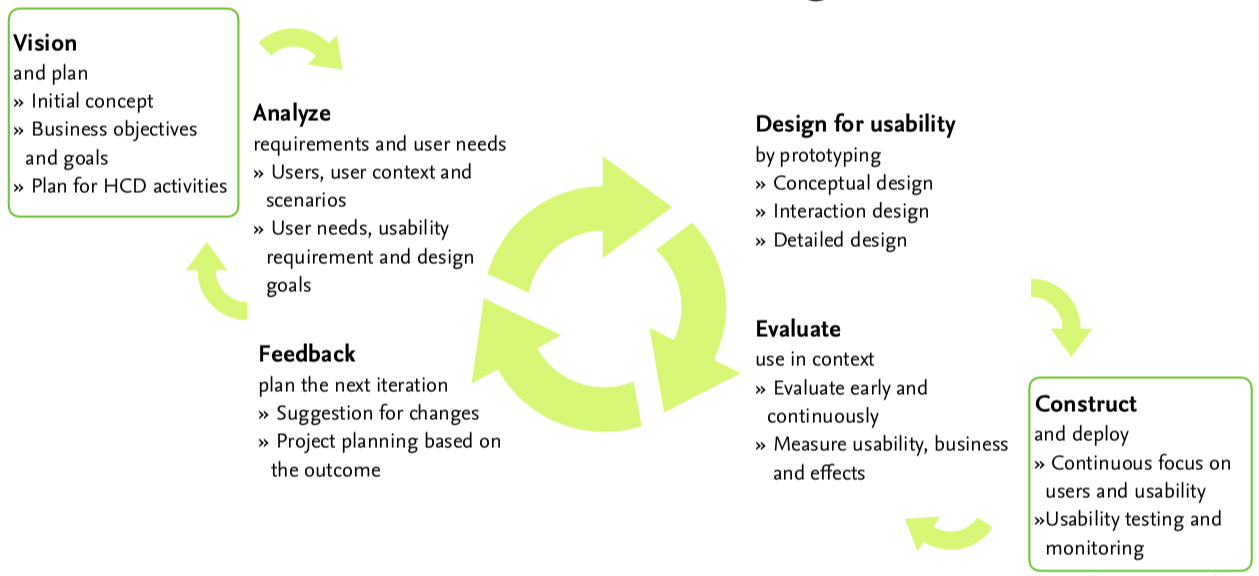
\includegraphics[width=\linewidth]{pics/hcd.png}
  \caption{User-centered System Design process by~\cite{gulliksenKeyPrinciplesUsercentred2003}}
\end{figure}

\begin{table}[htb]
\small
\colorbox{bamacolor}{
\centering
\begin{tabularx}{\textwidth}{@{} r Y @{}}
	&
	\textbf{Distinction between Bachelor and Master Thesis}\vspace{2mm}\\
    \textbf{B. Sc. Thesis} &
    The implementation phase is mandatory. \vspace{2mm}\\
	\textbf{M. Sc. Thesis} &
	The evaluation phase is mandatory. \vspace{2mm}\\

\end{tabularx}
}
\end{table}

Briefly describe the relevant planned steps of your HCD process in the following sections.

\subsection{Analyze}
\label{subsec:analyze}

\subsection{Design for Usability}
\label{subsec:design}

\subsection{Construct (Implementation)}
\label{subsec:implementation}

Especially in a B. Sc. thesis, an important part is the description of the technical concept. Even though in the proposal, this cannot be done in detail, the main libraries and the general architecture of the application should be outlined. Please use diagram types from the Unified Modeling Language (UML)\footnote{For further information, please check \url{https://en.wikipedia.org/wiki/Unified_Modeling_Language}.} for these details.

\subsection{Evaluation}
\label{subsec:evaluation}